\chapter{Metodología}
\label{ch:metodologia}

Este capítulo recoge la gestión del proyecto con un enfoque SCRUM adaptado a un TFM individual. Se busca dejar trazabilidad clara de qué se planificó, qué se ejecutó, qué bloqueos aparecieron y qué decisiones técnicas se tomaron en cada iteración.


\section{SCRUM adaptado a un desarrollo unipersonal}

SCRUM es una metodología ágil de carácter iterativo e incremental, orientada a organizar el trabajo en ciclos cortos, priorizar entregas de valor y revisar de forma continua el avance del producto \cite{ScrumGuide2020}. Aunque su formulación original está pensada para equipos, sus principios también pueden adaptarse a proyectos individuales cuando se busca mantener planificación, trazabilidad y capacidad de reacción ante cambios.

En este trabajo se ha utilizado una adaptación práctica de SCRUM, no como aplicación estricta del marco en todos sus elementos formales, sino como guía para estructurar el desarrollo del simulador, registrar decisiones y ordenar la evolución del proyecto. Esta adaptación ha resultado útil por tres motivos. En primer lugar, porque se han combinado tareas heterogéneas, incluyendo desarrollo backend, frontend, integración de motores de enrutado, tratamiento de datos, entrenamiento de modelos y redacción de memoria. En segundo lugar, porque el alcance real del proyecto ha ido evolucionando a medida que se validaban soluciones técnicas y se detectaban bloqueos. Por último, porque el seguimiento periódico con el tutor ha funcionado como mecanismo natural de revisión y reorientación.

Desde el punto de vista organizativo, la Guía Scrum 2020 define un \textit{Scrum Team} compuesto por tres responsabilidades principales: \textit{Product Owner}, \textit{Scrum Master} y \textit{Developers} \cite{ScrumGuide2020}. En un trabajo unipersonal esta separación no puede reproducirse de forma literal, por lo que se ha reinterpretado del siguiente modo:
\begin{itemize}
  \item \textbf{Product Owner}: el tutor académico ha asumido de forma aproximada esta función, al validar prioridades, orientar el alcance funcional del prototipo y revisar la utilidad de los entregables desde el punto de vista del objetivo del TFM.
  \item \textbf{Scrum Master}: esta responsabilidad ha sido asumida por el propio autor del trabajo, en la medida en que ha organizado iteraciones, registrado bloqueos, mantenido la trazabilidad del progreso y ajustado la planificación cuando han surgido incidencias técnicas o cambios de enfoque.
  \item \textbf{Developers}: el desarrollo técnico también ha recaído íntegramente en el autor, responsable de la implementación del simulador, la integración de servicios, el entrenamiento de modelos y la documentación de resultados.
\end{itemize}

En consecuencia, varias responsabilidades propias de un equipo Scrum han quedado concentradas en una única persona, mientras que el tutor ha actuado como agente externo de supervisión, validación y priorización. Esta circunstancia introduce diferencias claras respecto a un SCRUM de equipo, pero no invalida su uso como marco ligero de gestión. En este contexto, lo más relevante no ha sido reproducir todas las ceremonias de forma estricta, sino conservar los elementos que aportan valor real al proyecto: backlog priorizado, trabajo por iteraciones, revisión periódica y registro explícito de decisiones.

La metodología seguida en este trabajo se ha apoyado en los siguientes principios:
\begin{itemize}
  \item dividir el trabajo en sprints con objetivos acotados y entregables identificables;
  \item mantener un \textit{Product Backlog} vivo, revisado conforme avanzaba el proyecto;
  \item registrar en cada iteración qué se planificó, qué se completó y qué problemas aparecieron;
  \item utilizar las reuniones con el tutor como mecanismo de revisión y re-priorización;
  \item orientar cada sprint a la obtención de un incremento funcional o documental del proyecto.
\end{itemize}

En cuanto al seguimiento, las reuniones con el tutor comenzaron el 6 de noviembre de 2025 con la reunión de inicio del proyecto, con una cadencia aproximadamente quincenal durante el primer cuatrimestre. Tras una pausa en enero de 2026 coincidiendo con los exámenes, la frecuencia se intensificó a semanal a partir de febrero, con 19 sesiones celebradas entre enero y julio de 2026. Este ritmo de revisión periódica reforzó el carácter iterativo del proyecto y permitió alinear el trabajo de cada sprint con la retroalimentación del tutor, en particular durante los meses de mayor intensidad de desarrollo y escritura.

La Figura~\ref{fig:scrum_tfm_cycle} resume visualmente este ciclo de trabajo adaptado a un desarrollo unipersonal, mostrando la relación entre backlog, planificación, ejecución y revisión periódica con el tutor.

\begin{figure}[ht]
    \centering
    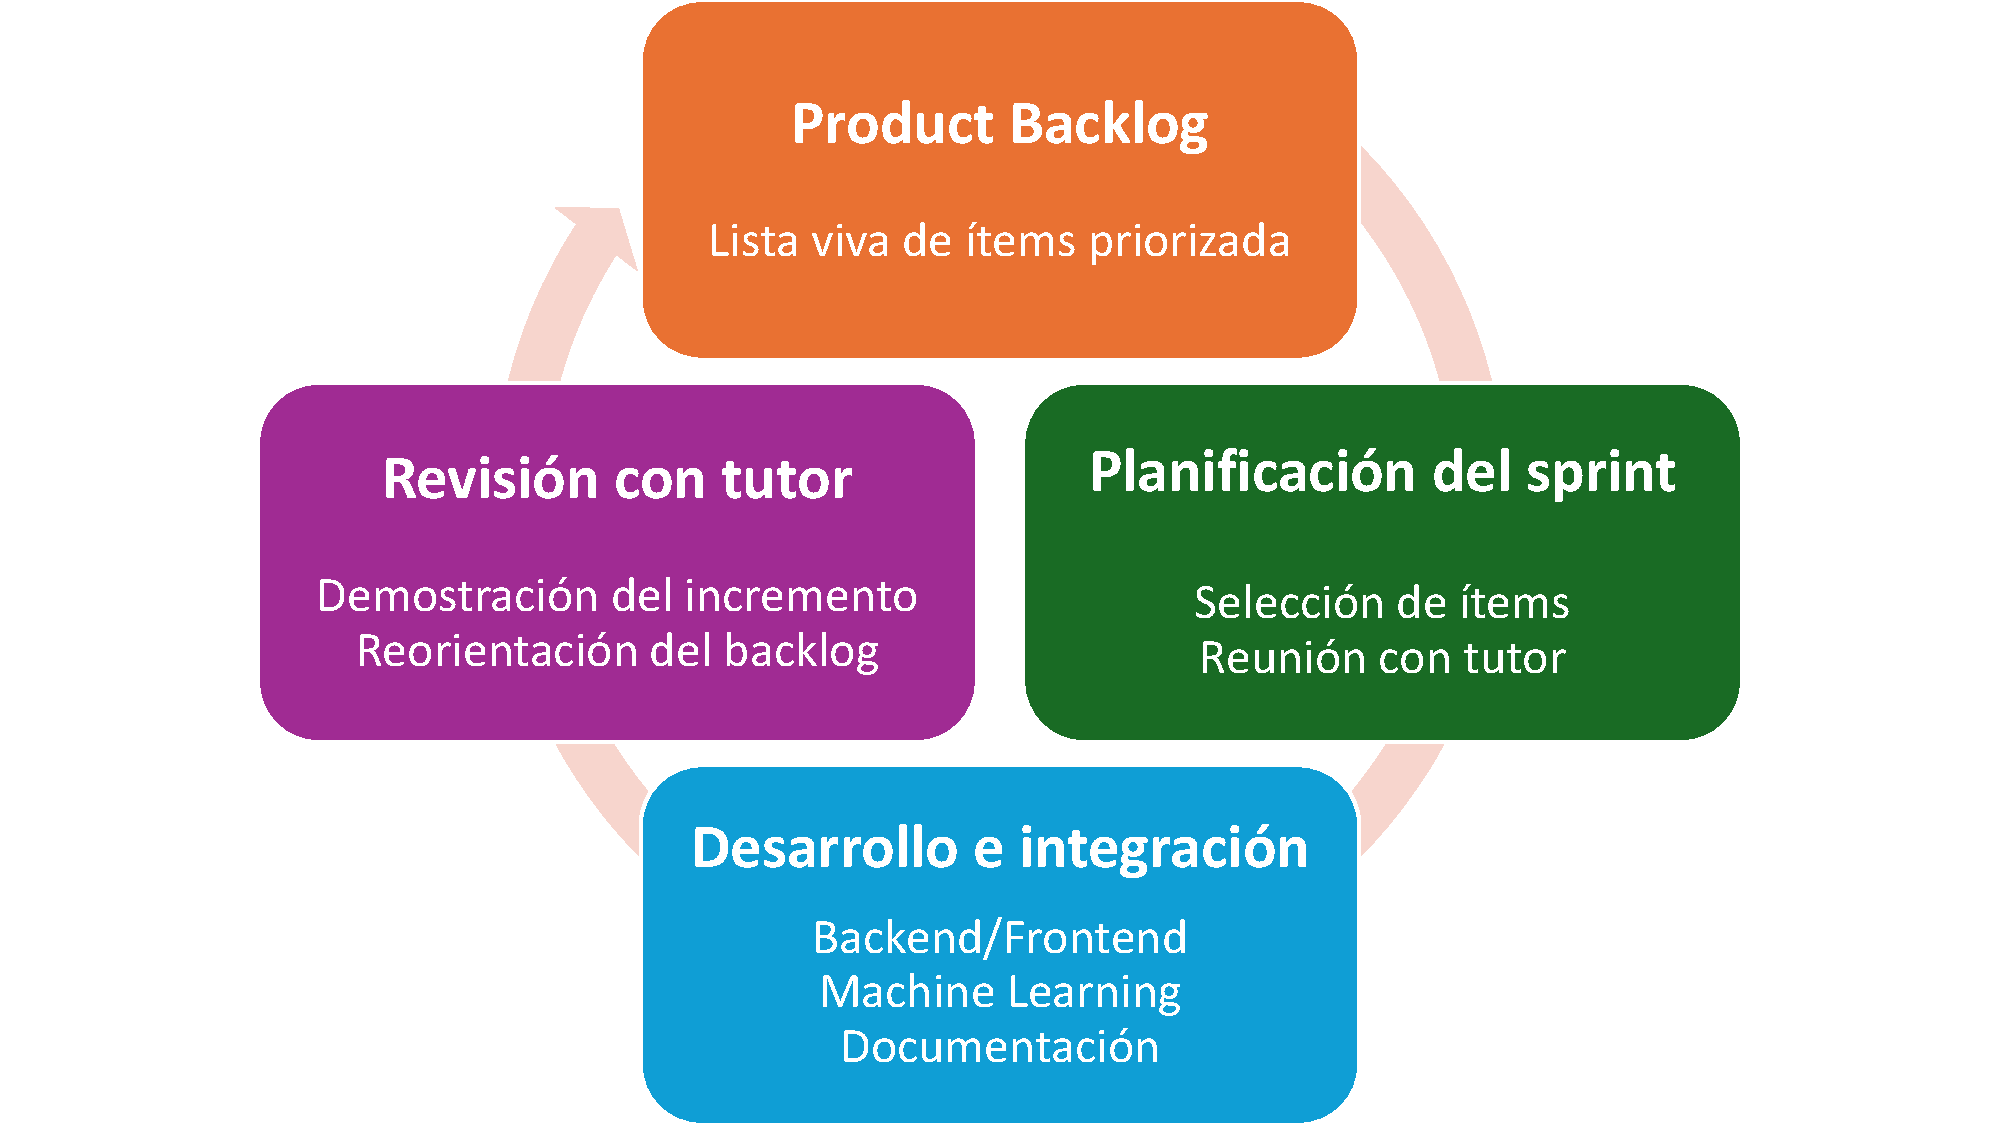
\includegraphics[width=1.1\textwidth]{figs/CicloSCRUMunipersonal.pdf}
    \caption{Esquema del ciclo de trabajo SCRUM adaptado al desarrollo unipersonal del proyecto. Elaboración propia.}
    \label{fig:scrum_tfm_cycle}
\end{figure}

Esta metodología ha encajado bien con la naturaleza del proyecto. Por una parte, ha permitido avanzar de manera incremental desde un prototipo inicial de rutas hasta un MVP funcional con integración de OSRM, OTP, GTFS y un modelo de elección modal. Por otra, ha facilitado documentar de forma ordenada tanto el trabajo ya completado como las líneas de evolución previstas, incluyendo mejoras visuales, ampliación de modelos y posibles análisis adicionales de simulación. A partir de este marco general, en los apartados siguientes se presenta el backlog del proyecto y el histórico de sprints ejecutados.
\newpage

\section{Product Backlog}

\subsection{Backlog inicial}

El \textit{Product Backlog} se definió como una lista viva de trabajo, organizada en grandes bloques funcionales y técnicos. En lugar de partir de un conjunto cerrado de tareas detalladas desde el inicio, se optó por un backlog de alto nivel que pudiera refinarse a medida que se validaban decisiones de diseño y se consolidaba el MVP del simulador.

En una primera aproximación, los elementos principales del backlog fueron los siguientes:

\begin{enumerate}
  \item Definir una arquitectura base cliente-servidor para desacoplar frontend, backend y servicios externos.
  \item Construir un prototipo web funcional con mapa interactivo, selección de origen-destino y visualización de rutas.
  \item Integrar OSRM en local con perfiles diferenciados para coche, bicicleta y desplazamiento a pie.
  \item Incorporar transporte público urbano mediante GTFS de Toledo y OpenTripPlanner.
  \item Diseñar una API propia que unifique consultas de rutas, exploración GTFS e inferencia modal.
  \item Preparar una pipeline reproducible de datos para el dataset LPMC.
  \item Entrenar y validar un primer modelo de elección modal utilizable dentro del simulador.
  \item Integrar el modelo de inferencia en backend y frontend de forma modular.
  \item Mejorar la interfaz, la experiencia de usuario y la capacidad de análisis visual del sistema.
  \item Documentar la solución, registrar la evolución del proyecto y redactar la memoria final.
\end{enumerate}

Conforme avanzó el trabajo, este backlog se fue refinando en tareas más concretas. Algunos elementos inicialmente planteados como trabajo futuro pasaron a formar parte del desarrollo principal, mientras que otros quedaron aplazados para iteraciones posteriores. A fecha de redacción de esta memoria, la parte nuclear del simulador puede considerarse ya implementada, por lo que el backlog actual se concentra principalmente en consolidación documental, mejoras visuales y ampliaciones funcionales sobre una base ya operativa.
\newpage

Para facilitar su seguimiento, los elementos del backlog se agruparon en cuatro bloques:
\begin{itemize}
  \item \textbf{Bloque funcional}: interfaz web, selección de viajes, cálculo de rutas, visualización de resultados y cuadro de información.
  \item \textbf{Bloque de integración de servicios}: despliegue y conexión de OSRM, OTP y GTFS dentro de una arquitectura reproducible.
  \item \textbf{Bloque de inteligencia artificial}: preprocesado del dataset LPMC, entrenamiento de modelos, validación e integración de inferencia.
  \item \textbf{Bloque documental y de cierre}: trazabilidad del proyecto, redacción de memoria, mejora de la presentación y preparación de resultados.
\end{itemize}


\subsection{Priorización de items}

La priorización del backlog no se realizó únicamente por orden técnico de implementación, sino por valor aportado al objetivo general del proyecto. En consecuencia, se siguió el siguiente criterio:
\begin{itemize}
  \item \textbf{Prioridad alta}: elementos necesarios para disponer de un simulador funcional extremo a extremo, incluyendo mapa interactivo, rutas por modo, integración de transporte público y una primera versión operativa de la inferencia modal.
  \item \textbf{Prioridad media}: mejoras que aumentan la usabilidad, la claridad visual o la trazabilidad del sistema, pero que no bloquean el funcionamiento básico del MVP.
  \item \textbf{Prioridad evolutiva}: ampliaciones previstas una vez estabilizado el núcleo del sistema, como el entrenamiento de modelos adicionales, la mejora de análisis de escenarios o la incorporación de nuevas visualizaciones y métricas.
\end{itemize}

Este criterio explica el orden seguido durante el desarrollo. Primero se priorizó la infraestructura mínima para obtener rutas y visualizar resultados reales sobre el mapa; después se incorporó el bloque de modelado e inferencia; y finalmente se abordaron tareas de consolidación, mejora y documentación. De esta forma, cada sprint pudo orientarse a producir incrementos útiles sobre una base ya validada, en lugar de avanzar en paralelo sobre demasiados frentes abiertos.
\newpage

\section{Histórico de sprints ejecutados}

En este apartado se resume la secuencia principal de trabajo seguida durante el desarrollo del proyecto. Los periodos y esfuerzos indicados se corresponden con la trazabilidad del historial de versiones, las reuniones de seguimiento y los artefactos generados, y deben interpretarse como estimaciones razonables. La carga de trabajo total del TFM asciende a 300 horas, correspondientes a los 12 ECTS del módulo; de ellas, aproximadamente 180 horas se orientaron al desarrollo técnico, 105 a la redacción de la memoria, 9 a las tutorías y 6 a la preparación de la defensa.

El cronograma completo en forma de diagrama de Gantt se recoge en el Anexo~\ref{anx:sprints}.

\subsection{Fase inicial: planificación y revisión del estado del arte}

\textbf{Fechas}: del 6 de noviembre al 19 de diciembre de 2025.

\textbf{Esfuerzo estimado}: 10--14 horas, incluyendo tutorías y trabajo exploratorio previo al primer sprint.

Antes de iniciar el desarrollo técnico se celebraron seis reuniones con el tutor que sirvieron para definir el alcance del proyecto, revisar el estado del arte y acordar la estructura metodológica. La reunión de inicio (6 de noviembre, 80 minutos) estableció el marco general: un simulador web de movilidad urbana centrado en Toledo, con OSRM y OTP como motores de enrutado, GTFS como fuente de la red de transporte público y un modelo de elección modal entrenado sobre el dataset LPMC, proporcionado por el tutor. Las dos sesiones siguientes (14 y 24 de noviembre) sirvieron para revisar trabajos de referencia sobre modelado de elección discreta y aprendizaje automático aplicado a movilidad, y para explorar las opciones de pila tecnológica disponibles.

La reunión del 4 de diciembre coincidió con la primera sesión de estado del arte formal y también con los primeros commits del repositorio: un PoC inicial con FastAPI y React que ya incluía integración con OSRM remoto y visualización de rutas en el mapa. Las reuniones del 11 de diciembre (metodología) y el 19 de diciembre (planificación) cerraron esta fase con el acuerdo sobre el proceso de desarrollo mediante SCRUM adaptado y la definición de los primeros bloques de trabajo del backlog.

El resultado de esta fase fue, por tanto, doble: por un lado, la validación técnica preliminar de las tecnologías clave a través del PoC; por otro, la definición del alcance, la metodología y la estructura iterativa que guió los catorce sprints posteriores.

\subsection{Sprint 1: Validación inicial de OSRM mediante servicios remotos}

\textbf{Fechas}: del 4 al 9 de diciembre de 2025.

\textbf{Esfuerzo estimado}: 8--12 horas.

Este sprint tuvo como objetivo investigar distintas herramientas de enrutado y, en particular, validar la viabilidad de OSRM dentro del proyecto mediante llamadas remotas desde una primera arquitectura cliente-servidor. El propósito no era todavía disponer de una solución definitiva, sino comprobar que el flujo completo entre mapa, backend y cálculo de rutas resultaba técnicamente factible.

El principal resultado de esta iteración fue la construcción de un primer prototipo funcional y la identificación temprana de las limitaciones de los servicios remotos utilizados para las pruebas iniciales. Esta validación permitió confirmar el interés de OSRM como base del simulador, pero también puso de manifiesto la necesidad de avanzar hacia una infraestructura propia para garantizar comparabilidad real entre modos y mayor control experimental.

\subsection{Sprint 2: Despliegue del servicio OSRM local multi-perfil}

\textbf{Fechas}: del 4 al 10 de diciembre de 2025.

\textbf{Esfuerzo estimado}: 12--16 horas.

Una vez validado el uso de OSRM para este trabajo, este sprint se orientó al despliegue de una instancia local que permitiera obtener rutas diferenciadas para distintos modos de desplazamiento y, al mismo tiempo, mantener un control total sobre la infraestructura. Este cambio era necesario para asegurar reproducibilidad, trazabilidad y estabilidad en las comparaciones realizadas por el simulador.

Como resultado, el proyecto dejó de depender de servicios públicos externos y pasó a apoyarse en una base de cálculo local sobre la que posteriormente se construirían tanto la comparación modal como la integración con el resto de componentes del sistema.

\subsection{Sprint 3: Incorporación del GTFS urbano de Toledo}

\textbf{Fechas}: del 11 al 14 de diciembre de 2025.

\textbf{Esfuerzo estimado}: 10--14 horas.

El objetivo de esta iteración fue incorporar la red de transporte público urbano de Toledo al simulador a partir del feed GTFS descargado desde el Punto de Acceso Nacional (NAP) del Ministerio de Transportes. Para ello se desarrolló el módulo de lectura \texttt{gtfs\_loader.py}, que parsea y mantiene en memoria la información de paradas, rutas, viajes y horarios, y se implementaron cuatro endpoints en el router \texttt{/api/gtfs}: listado de paradas con filtro opcional por bounding box, listado de líneas de la red, detalle de ruta con paradas ordenadas y trazado geométrico, y resumen de horarios por fecha.

En la capa de visualización se añadieron las paradas como marcadores circulares en el mapa con popup interactivo, desde el que el usuario puede consultar qué líneas dan servicio en cada parada. Este sprint no incluyó planificación de itinerarios, que se abordó en el sprint siguiente. Su resultado principal fue disponer de una representación operativa completa de la red de bus urbano de Toledo, desacoplada del grafo OTP, lo que permite consultar la red aunque el planificador no esté disponible.

\subsection{Sprint 4: Integración de OpenTripPlanner para rutas multimodales}

\textbf{Fechas}: del 11 de diciembre de 2025 al 12 de febrero de 2026.

\textbf{Esfuerzo estimado}: 16--24 horas.

Tras la incorporación del GTFS, este sprint se centró en habilitar el cálculo de rutas de transporte público puerta a puerta mediante OpenTripPlanner. El objetivo era pasar de una visualización estática de red a una capacidad real de planificación multimodal, incorporando la combinación entre red peatonal y servicio de autobús urbano.

Esta fase supuso un salto cualitativo dentro del proyecto, ya que permitió integrar en una misma aplicación los modos viarios y el modo tránsito, haciendo posible una comparación más completa entre alternativas de viaje en el contexto urbano de Toledo.

\subsection{Sprint 5: Diseño de la interfaz web y codificación visual por modo}

\textbf{Fechas}: del 11 de diciembre de 2025 al 20 de febrero de 2026.

\textbf{Esfuerzo estimado}: 8--12 horas.

Este sprint se orientó a consolidar la experiencia de usuario y la legibilidad comparada de resultados. Las principales decisiones de diseño adoptadas fueron: codificación visual de rutas por modo (azul sólido para conducción, verde sólido para bicicleta y gris discontinuo para desplazamiento a pie); visualización de segmentos OTP diferenciada entre tramos en vehículo, representados en naranja, y tramos a pie, con la misma trama discontinua que el modo peatonal; basemaps seleccionables por el usuario; y marcadores SVG personalizados para origen y destino con iconografía diferenciada.

Se consolidó también el uso de TanStack Query para las peticiones al backend, que proporciona caché de respuestas, gestión declarativa de estados de carga y reintento automático en caso de error. Los segmentos de transporte público se restringieron a modo \textit{transit}, evitando solapamientos visuales con las rutas viarias. El resultado fue una interfaz directamente utilizable como herramienta de análisis, no solo como demostración técnica del sistema de enrutado.

\subsection{Sprint 6: Diseño de un modelo de clasificación de modo de viaje y procesado de datos}

\textbf{Fechas}: del 21 de diciembre de 2025 al 17 de enero de 2026.

\textbf{Esfuerzo estimado}: 12--18 horas.

Este sprint tuvo como finalidad preparar la base metodológica del módulo de inteligencia artificial del proyecto. Para ello se abordó el estudio del dataset LPMC, la revisión de trabajos de referencia y el diseño del proceso de preparación de datos necesario para entrenar modelos de clasificación de modo de viaje con un criterio reproducible.

El trabajo realizado en esta fase no se orientó todavía a la integración en el simulador, sino a establecer una base sólida de modelado sobre la que poder entrenar, comparar y validar distintos enfoques en iteraciones posteriores.

\subsection{Sprint 7: Entrenamiento y validación de los modelos de clasificación}

\textbf{Fechas}: del 18 de enero al 21 de febrero de 2026.

\textbf{Esfuerzo estimado}: 14--20 horas.

Una vez definida la base de datos y el proceso de preparación, este sprint se centró en entrenar y validar los primeros modelos de clasificación de modo de viaje. El objetivo fue disponer de una referencia cuantitativa útil, suficientemente estable como para servir de punto de partida a la integración del módulo de inferencia dentro del simulador.

Como resultado, el proyecto avanzó desde una fase exploratoria sobre datos hacia una fase claramente aplicada, en la que ya era posible valorar el rendimiento de los modelos y decidir cuáles podían incorporarse al sistema de forma operativa.

\subsection{Sprint 8: Escritura de la memoria y consolidación metodológica}

\textbf{Fechas}: del 27 de enero al 23 de junio de 2026, en paralelo al resto de sprints técnicos.

\textbf{Esfuerzo estimado}: 60--80 horas distribuidas a lo largo de los cinco meses de redacción activa.

La escritura de la memoria no se desarrolló como una actividad aislada al final del proyecto, sino como una línea de trabajo transversal que se extendió de forma continua desde el inicio del segundo cuatrimestre hasta la semana previa al depósito. En su arranque (enero--marzo de 2026) el objetivo fue consolidar la estructura documental del TFM y fijar el enfoque de cada capítulo; en su fase de desarrollo (abril--mayo), alinear la narración con las decisiones técnicas adoptadas en cada iteración; y en su cierre (junio), completar y revisar el conjunto de la memoria antes de la preparación del depósito.

La redacción estuvo estrechamente ligada al calendario de reuniones con el tutor: las sesiones de revisión de memoria de abril y mayo de 2026 marcaron las entregas parciales de los capítulos 4 y 5, mientras que las revisiones de junio sirvieron para contrastar el texto con el estado definitivo de la aplicación y corregir las incoherencias detectadas. Este sprint debe interpretarse, por tanto, como un esfuerzo acumulativo distribuido y no como una fase puntual de escritura.

\subsection{Sprint 9: Integración del módulo de inferencia en el simulador}

\textbf{Fechas}: del 21 de febrero al 8 de marzo de 2026.

\textbf{Esfuerzo estimado}: 14--20 horas.

El objetivo de esta iteración fue integrar el módulo de inferencia modal dentro del simulador ya construido, conectando el bloque de modelado con la aplicación web y con la lógica general del backend. Con ello se buscaba que el sistema dejara de ser únicamente un comparador de rutas para incorporar también una capa predictiva sobre la elección de modo de viaje.

Esta integración representó la convergencia de las dos grandes líneas del TFM: por un lado, la construcción del simulador de movilidad urbana; por otro, el diseño y validación de modelos de clasificación. A partir de este punto, el proyecto quedó configurado como una aplicación capaz de combinar cálculo de rutas, visualización cartográfica e inferencia modal en un mismo entorno de trabajo.

\subsection{Sprint 10: Reestructuración del repositorio y documentación de la arquitectura}

\textbf{Fechas}: del 17 de marzo al 15 de abril de 2026.

\textbf{Esfuerzo estimado}: 14--20 horas.

El proyecto presentaba una deuda técnica acumulada: los distintos componentes, incluyendo backend, frontend, scripts de entrenamiento y configuración Docker, se habían desarrollado de forma incremental y necesitaban unificarse en un repositorio coherente para la entrega final. Este sprint abordó esa consolidación integrando todos los módulos en un monorrepo con estructura clara de directorios y preparando la documentación técnica para la fase de escritura del capítulo de arquitectura.

La tarea documental más relevante fue la redacción del capítulo 4, que formalizó las decisiones de diseño acumuladas durante los sprints anteriores: la tabla de servicios Docker, los cuatro grupos de endpoints de la API, el diagrama del pipeline de inferencia y la descripción de la capa de orquestación. Documentar la arquitectura antes de entrar en el detalle del capítulo 5 permitió detectar algunas inconsistencias menores en los contratos de la API y corregirlas antes de que quedaran fijadas en la memoria.

\subsection{Sprint 11: Entrenamiento de modelos adicionales y comparativa multi-modelo}

\textbf{Fechas}: del 28 de abril al 6 de mayo de 2026.

\textbf{Esfuerzo estimado}: 20--28 horas.

El bloque de inteligencia artificial contaba en ese momento únicamente con el modelo XGBoost entrenado en el sprint 7. Este sprint amplió el repertorio con un segundo modelo de tipo bosque aleatorio (Random Forest) y un tercero de red neuronal profunda implementado en PyTorch mediante un módulo \texttt{TorchModalWrapper}, lo que permitió comparar tres enfoques de aprendizaje automático sobre el mismo dataset LPMC y el mismo conjunto de variables de entrada. En los tres modelos se aplicó validación cruzada con GroupKFold, agrupando por identificador de hogar para evitar que viajes de un mismo hogar aparecieran simultáneamente en los conjuntos de entrenamiento y de test.

Durante esta fase se detectó y corrigió un error en el pipeline de inferencia: las duraciones de ruta devueltas por OSRM y OTP estaban en segundos, mientras que el dataset LPMC las registra en horas. Sin esa conversión, las duraciones llegaban al modelo con un factor de inflación de 3.600, lo que distorsionaba completamente las predicciones. La corrección se aplicó tanto en el módulo de entrenamiento como en el de inferencia. Se añadió también el endpoint \texttt{POST /api/lpmc/compare}, que ejecuta los tres modelos en paralelo y devuelve sus probabilidades de forma comparada, junto con el panel de comparación correspondiente en el frontend.

\subsection{Sprint 12: Redacción del capítulo de implementación y primer rediseño de la interfaz}

\textbf{Fechas}: del 19 de mayo al 10 de junio de 2026.

\textbf{Esfuerzo estimado}: 28--36 horas.

Este sprint combinó dos líneas de trabajo en paralelo. Por un lado, la redacción de las seis secciones del capítulo 5, que recorren la implementación de OSRM, OTP, el módulo GTFS, el backend FastAPI, el frontend React y el bloque de modelado. La escritura en detalle de cada sección exigió revisar el estado real del código y, en varios casos, corregir implementaciones que habían quedado incompletas o cuya documentación no reflejaba su funcionamiento real.

Por otro lado, la interfaz recibió su primer rediseño estructural: se sustituyó el diseño anterior por un sidebar-rail fijo de 64 píxeles con cuatro paneles funcionales (Rutas, Red de transporte, Predicción IA y Capas) que flotan sobre el mapa sin desplazarlo. Se incorporó un menú contextual al hacer clic derecho sobre el mapa para establecer el origen o el destino del viaje. Se activó además el Plan A de manejo de itinerarios sin transporte público real: cuando OTP no devuelve ningún tramo de bus, las variables de transporte público se sustituyen por valores de penalización extremos antes de la inferencia, de forma que el modelo descarte esa alternativa por sus propias reglas sin necesidad de intervención posterior.

\subsection{Sprint 13: Consolidación de la interfaz y preparación del repositorio para entrega}

\textbf{Fechas}: del 11 al 25 de junio de 2026.

\textbf{Esfuerzo estimado}: 30--40 horas.

Este sprint agrupó dos semanas de mejoras de interfaz, infraestructura y documentación orientadas a dejar el sistema en el estado que se presenta en la defensa. En la parte visual, el panel de la red GTFS fue rediseñado por completo: las líneas se agrupan por nombre corto en un acordeón desplegable con un diagrama de paradas al estilo de un cartel de línea, y se garantizan colores únicos asignando una paleta de 26 tonos a las 25 líneas del feed de Toledo por índice alfabético. Se añadió un panel de Ajustes con un selector de modelo activo que carga las opciones dinámicamente desde la API sin necesidad de reiniciar el contenedor, resolviendo una dependencia que hasta entonces requería edición manual de la variable de entorno. Se sustituyeron también los controles de zoom nativos de Leaflet por componentes React con lógica de limpieza de rutas, se instaló la librería Lucide React para la iconografía de la interfaz y se añadió un panel de Inicio con la descripción del proyecto y los créditos.

En cuanto a la infraestructura, el repositorio se reorganizó para la entrega pública: se configuró Git LFS para los artefactos pesados (grafos OSRM, grafo OTP, fichero GTFS ZIP y modelos ML), se añadieron servicios de inicialización idempotentes en Docker Compose para que el sistema arranque correctamente en cualquier máquina sin pasos manuales, y se redactaron los ficheros README en inglés y español. El repositorio fue renombrado a \texttt{movilidad-urbana} en GitHub.

En los últimos días del sprint (24--25 de junio) se cerraron además varios flecos técnicos y documentales relevantes. Se resolvió un error de resolución de la línea de bus en el panel Rutas causado por el prefijo del feedId que OTP añade al route\_id (ej. \texttt{1:50011}); las insignias de color ahora resuelven la ruta por id exacto, sin prefijo, o por nombre corto. Se reconstruyó el grafo de OTP con el feed GTFS\_Urbano\_Toledo\_2026 (22 de febrero a 22 de mayo de 2026), eliminando el feed de diciembre de 2025 que causaba incoherencia entre el planificador y el panel de red estática. Se unificó el control de fecha y hora del viaje en un único elemento permanente sobre el mapa, eliminando los controles independientes que existían en tres paneles distintos. Se corrigió también un error de zona horaria en las horas mostradas, que se debía a que el campo de tiempo de OTP se expresaba en UTC y no se aplicaba el desplazamiento de la agencia. Los puertos de los servicios OSRM en el host se actualizaron de 5000/5001/5002 a 5001/5002/5003 para evitar el conflicto con AirPlay en macOS. Y se realizó una primera revisión integral de los capítulos 4 y 5 contrastándolos con el estado final de la aplicación, junto con la creación de los cuatro anexos de la memoria (manual de despliegue, contratos de la API, configuración experimental y evidencias de sprints).

\subsection{Sprint 14: Pulido final de la aplicación y revisión integral de la memoria}

\textbf{Fechas}: del 28 de junio al 6 de julio de 2026.

\textbf{Esfuerzo estimado}: 20--26 horas.

El último sprint del proyecto concentró el trabajo de revisión final y cierre previo al depósito. La semana del 28 de junio al 6 de julio incluyó dos pasadas de revisión estructural de la memoria. En la segunda pasada (30 de junio) se añadieron las búsquedas de hiperparámetros propias para los modelos Random Forest y DNN, implementadas respectivamente en \texttt{lpmc/04\_tune\_rf.py} (HyperOpt/TPE, 100 evaluaciones) y \texttt{lpmc/05\_tune\_dnn.py} (búsqueda aleatoria, 30 configuraciones), y se retrenaron ambos modelos con los parámetros hallados: RF final con 500 árboles, profundidad máxima 20, mínimo 15 muestras por nodo interno y 6 por hoja; DNN final con capas ocultas 128-128-64, tasa de aprendizaje $3\times10^{-3}$ y dropout 0.3/0.2. El módulo \texttt{TorchModalWrapper} del backend se actualizó para reconstruir la arquitectura de la red directamente desde los metadatos del checkpoint, eliminando la configuración hardcodeada anterior. En la tercera pasada (también 30 de junio) se realizó una reorganización estructural del capítulo 4 (\S4.2 renombrada a ``Infraestructura, orquestación y portabilidad''; \S4.3 a ``Backend: API y routers'') y del capítulo 5 (\S5.2 reordenada y renombrada; \S5.3 eliminada por absorción en \S5.2; nueva \S5.6.5 sobre ajustes y conocimiento experto). Tras estas revisiones la memoria compilaba limpia con XeLaTeX en 115 páginas.

La reunión del 1 de julio sirvió para revisar el estado del depósito y la lista de elementos pendientes: redacción de los agradecimientos, resumen en inglés y las capturas de pantalla finales de la interfaz. Los días 5 y 6 de julio se completó una primera revisión integral de todo el documento, con correcciones de contenido en los capítulos 1, 3 y los anexos, y la actualización del diagrama de Gantt y de las figuras vectoriales del capítulo 3.


\section{Retrospectiva del ciclo de desarrollo}

\subsection{Aprendizajes por iteración}

El desarrollo del proyecto dejó cinco aprendizajes técnicos que merecen recogerse explícitamente, tanto por su impacto real sobre el trabajo como por su aplicabilidad en proyectos similares:

\begin{itemize}
  \item \textbf{Validar los servicios externos en una iteración temprana y aislada evita retrabajo costoso.} El descubrimiento en el sprint 1 de que el servidor de demostración de OSRM solo ofrece el perfil de conducción motivó la transición inmediata a una infraestructura local, que fue la base de todo el desarrollo posterior. Posponer esa validación al sprint 5 o posterior habría obligado a replantear la arquitectura cuando ya existía código construido sobre ella.

  \item \textbf{La coherencia entre las unidades de los datos de entrada y las del dataset de entrenamiento es un invariante crítico en cualquier pipeline de inferencia.} El factor de conversión de segundos a horas entre las salidas de OSRM/OTP y el dataset LPMC pasó desapercibido durante varios sprints y produjo predicciones completamente incorrectas hasta su detección y corrección en el sprint 11. Documentar las unidades esperadas por el modelo junto a la definición de cada variable habría evitado el error desde el principio.

  \item \textbf{Cuando dos componentes dependen del mismo conjunto de datos con mecanismos de carga distintos, es necesario mantener un único punto de referencia temporal.} La coexistencia del feed GTFS de diciembre de 2025 en el grafo de OTP con el feed de 2026 en el módulo de consulta estática creó una incoherencia que solo se detectó al intentar visualizar horarios para las mismas fechas en ambos componentes. La lección es verificar la consistencia temporal de los datos entre servicios antes de integrarlos en la interfaz de usuario.

  \item \textbf{Las técnicas de evaluación de modelos de clasificación pueden introducir data leakage si no se tiene en cuenta la estructura jerárquica de los datos.} En el dataset LPMC varios miembros de un mismo hogar realizaron viajes distintos; sin el uso de GroupKFold agrupado por identificador de hogar, viajes del mismo hogar podían aparecer simultáneamente en los conjuntos de entrenamiento y de test, inflando artificialmente las métricas de evaluación. El split temporal por survey year era necesario pero insuficiente por sí solo.

  \item \textbf{Registrar las decisiones de diseño en la memoria en paralelo al desarrollo acelera la redacción final y reduce la pérdida de contexto técnico.} Las secciones del capítulo 5 que más tiempo requirieron fueron precisamente aquellas para las que no se había dejado trazabilidad escrita durante los sprints correspondientes. Las secciones redactadas inmediatamente después de completar su implementación resultaron más precisas y requirieron menos revisión.
\end{itemize}

\subsection{Acciones de mejora aplicadas}

En respuesta a los aprendizajes anteriores, se tomaron las siguientes acciones correctoras:

\begin{itemize}
  \item Se migró a OSRM local en el sprint 2, inmediatamente después de identificar las limitaciones del servidor público, sin esperar a que el problema bloqueara fases más avanzadas del desarrollo.
  \item Se añadió la conversión explícita de segundos a horas en el módulo de inferencia, se documentó el invariante en el código y se verificó de forma explícita que los scripts de entrenamiento y el servicio de predicción aplicaran el mismo factor de escala.
  \item El grafo de OTP se reconstruyó con el feed de 2026 y se eliminó el feed antiguo del repositorio, garantizando que ambos componentes operaran sobre la misma ventana temporal.
  \item Se incorporó GroupKFold con el identificador de hogar como criterio de agrupación en el entrenamiento de los tres modelos, y se mantuvo el split temporal por survey year como criterio de partición del conjunto de evaluación.
  \item Se estableció la práctica de actualizar la memoria al cierre de cada sprint con las decisiones técnicas más relevantes, reduciendo la carga documental en la fase final y mejorando la precisión de las secciones de implementación.
\end{itemize}


\section{Cierre del ciclo de desarrollo}
\label{sec:scrum_cierre}

El proceso comenzó con una fase inicial de planificación y revisión del estado del arte que abarcó de noviembre a diciembre de 2025, seguida de la secuencia de catorce sprints descrita en este capítulo. El conjunto llevó el proyecto desde la validación tecnológica inicial hasta un simulador funcional completo, con integración de rutas viarias, transporte público multimodal, red GTFS estática, inferencia de elección modal mediante tres modelos de aprendizaje automático y una interfaz de usuario lista para su presentación.

El desarrollo puede dividirse en tres fases diferenciadas. Una primera fase de infraestructura y validación tecnológica (sprints 1 a 5) orientada a demostrar la viabilidad del sistema y establecer la arquitectura de integración de servicios. Una segunda fase de desarrollo del bloque de inteligencia artificial (sprints 6, 7, 9 y 11), centrada en el procesamiento del dataset LPMC, el entrenamiento de tres modelos de clasificación y su integración en la API del sistema. Una tercera fase de consolidación, pulido visual y documentación (sprints 8, 10, 12, 13 y 14), en la que el simulador alcanzó su forma definitiva y la memoria fue redactada y revisada. Las fases primera y segunda se solapan temporalmente en varios meses, reflejo del carácter iterativo del desarrollo y de la necesidad de avanzar en paralelo sobre la infraestructura y el bloque de modelado.

La arquitectura resultante y las decisiones técnicas adoptadas a lo largo de este proceso se describen en el capítulo~\ref{ch:arquitectura}. Los detalles de implementación de cada componente se recogen en el capítulo~\ref{ch:implementacion}.
